\documentclass[serif]{beamer}  % for 4:3 ratio

% Encoding & packages
\usepackage[utf8]{inputenc}
\usepackage[T1]{fontenc} 
\usepackage{hyperref}
\usepackage{latexsym,amsmath,xcolor,multicol,booktabs,calligra}
\usepackage{graphicx,listings,stackengine}
\usepackage{UoWstyle}

% Author/title info
\author{
    Giovanni Billo
    \and  
    Andrea Suklan
    \and  
    Carlos Velázquez Fernández
}
\title{Analysis of RL Algorithms for a Simulated Hill Climb Racing Agent}
\date{\small July 28, 2025}

% Custom commands and colors
\def\cmd#1{\texttt{\color{red}\footnotesize $\backslash$#1}}
\def\env#1{\texttt{\color{blue}\footnotesize #1}}
\definecolor{deepblue}{rgb}{0,0,0.5}
\definecolor{deepred}{RGB}{153,0,0}
\definecolor{deepgreen}{rgb}{0,0.5,0}
\definecolor{halfgray}{gray}{0.55}

% Code listing setup
\lstset{
    basicstyle=\ttfamily\tiny,
    keywordstyle=\bfseries\color{deepgreen},
    emphstyle=\ttfamily\color{deepred},
    stringstyle=\color{deepblue},
    numbers=left,
    numberstyle=\tiny\color{halfgray},
    rulesepcolor=\color{red!20!green!20!blue!20},
    frame=shadowbox,
}

\begin{document}

\begin{frame}
    \vfill
    \begin{center}
        
\includegraphics[keepaspectratio, scale=0.15]{images/logo.jpg}
        \vspace{1cm}
        \begin{beamercolorbox}[wd=\textwidth,center,rounded=true]{title}
            \textbf{Analysis of RL Algorithms for \\ a Simulated Hill Climb Racing Agent}
        \end{beamercolorbox}
        \vspace{1cm}
        {July 28, 2025}
    \end{center}
    \vfill
\end{frame} 

\begin{frame}    
\tableofcontents[sectionstyle=show,
subsectionstyle=show/shaded/hide,
subsubsectionstyle=show/shaded/hide]
\end{frame}

\section{Introduction}

\section{Environment}

\section{Deep Q-Network}

\begin{frame}{Based on Q-Learning}
    \begin{figure}
        \centering
        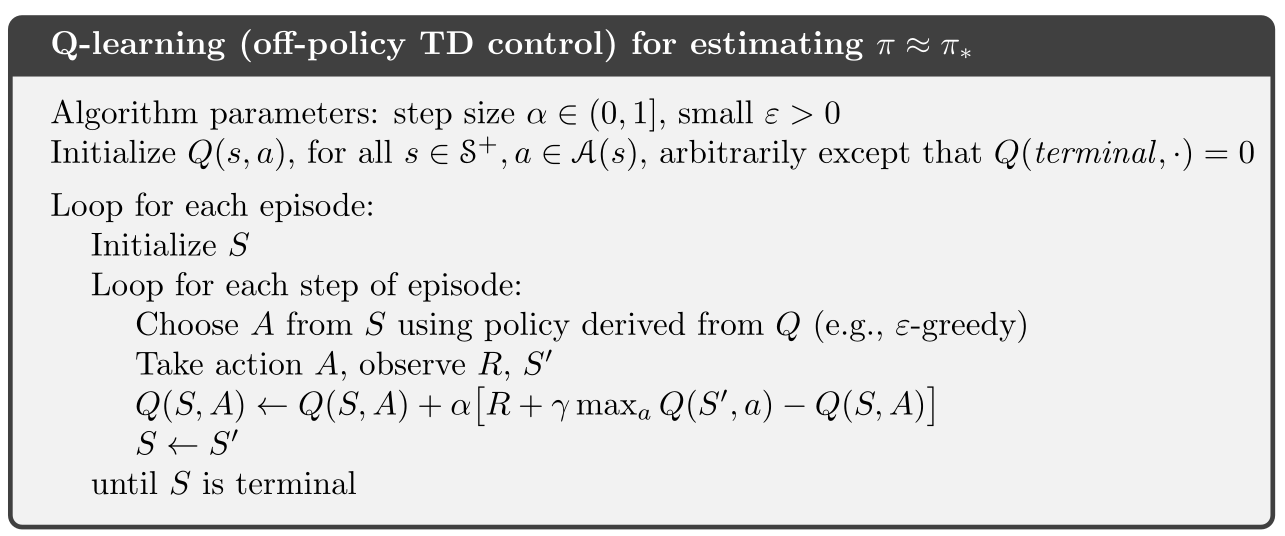
\includegraphics[width=\linewidth]{images/Q_LEARNING_ALGO.png}
    \end{figure}
    \begin{itemize}
        \item Model-Free (separate Prediction and Control) 
        \item Off-Policy
        \item $\epsilon$-greedy policy (with decay)
    \end{itemize}
\end{frame}

\begin{frame}{DQN Algorithm}
    \begin{figure}
        \centering
        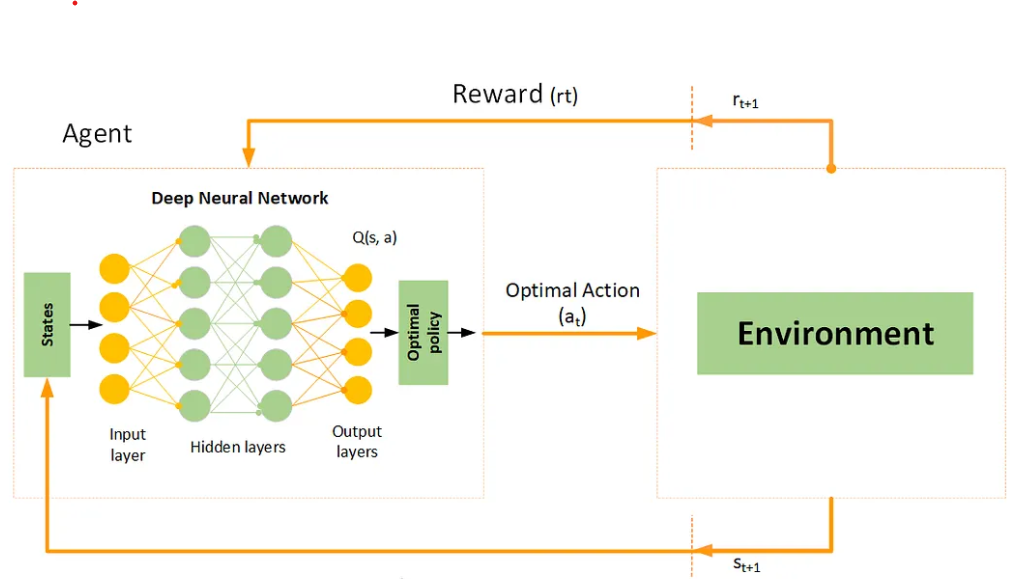
\includegraphics[width=\linewidth]{images/DQN_diagram.png}
    \end{figure}
    \begin{itemize}
        \item Semi-Gradient Method: $\hat{q}(s, a, \mathbf{w}) \approx q_{\star}(s, a), \mathbf{w} \in \mathbb{R}$ 
        \item Uses \textit{Replay Buffer} to tackle the \textit{moving target problem}.  
    \end{itemize}
\end{frame}

\begin{frame}{More specifically}
    \textbf{Weight update in DQN}
    $$
    \mathbf{w} \leftarrow \mathbf{w} + \alpha \left[ R + \gamma \max_{A'} \hat{q}(S', A', \mathbf{w}^{-}) - \hat{q}(S, A, \mathbf{w}) \right] \nabla \hat{q}(S, A, \mathbf{w})
    $$
\end{frame}

\section{Expected SARSA}

\begin{frame}{Expected SARSA Algorithm}
    \begin{figure}
        \centering
        \includegraphics[width=\linewidth]{images/ESARSA_diagram.png}
    \end{figure}
\end{frame}

\section{Proximal Policy Optimization}

\begin{frame}{PPO Algorithm}
    \begin{figure}
        \centering
        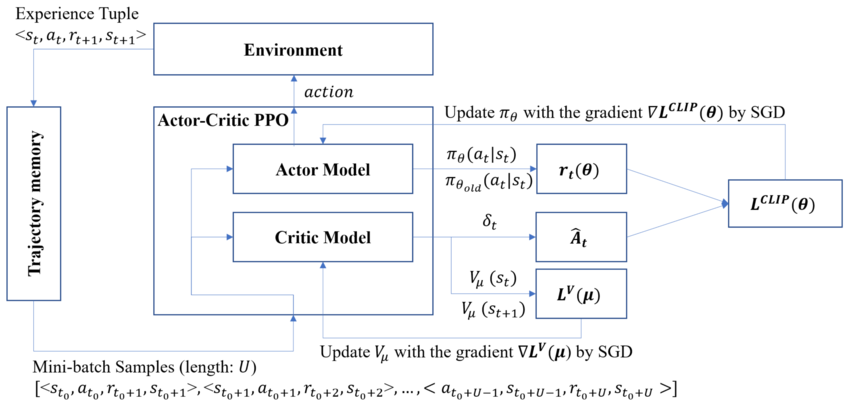
\includegraphics[width=\linewidth]{images/PPO_diagram.png}
    \end{figure}
\end{frame}

\section{Results}

\begin{frame}
\centering
{\Huge Thank you!}
\end{frame}

\bibliography{ref}
\bibliographystyle{plain}

\end{document}

